\chapter{Compiler Integration}
\label{chap:compilerintegration}

In diesem Kapitel wird beschrieben, wie der Compiler in die Entwicklungsumgebung eingebunden wurde um ein C-File nach Forth zu übersetzten. Und welche Möglichkeiten mit dem CDT für das Editieren von C-Files zur Verfügung stehen.

\section{Integration im Eclipse CDT}

Das CDT stellt Extension Points zur Verfügung, welche gebraucht werden können um einen Compiler zu integrieren. Diese Extension Points werden in den nächsten Kapitel erläutert und es wird erklärt wie der LCC dadurch in die Entwicklungsumgebung eingebunden wird.

\subsection{Configuration Beschreibung}
Eine Konfiguration wird gebraucht um verschiedene Standard Tools und Optionen bereit zu stellen, um ein Projekt auf eine gewisse Weise zu kompilieren. Normalerweise existieren für ein Projekt zwei Konfigurationen. Eine Debug- und eine Releasekonfiguration.

\subsection{Configuration Verwendung}
Für die Entwicklungsumgebung gibt nur eine Konfiguration für den Release Build. Debug spezifische Files werden von dem Launch generiert, da der Kompiler damit nichts zu tun hat.

\subsection{Tool Beschreibung}
Definiert ein Tool, wie zum Beispiel ein Compiler oder Linker, welches verwendet wird im Buildprozess.

\subsection{Tool Verwendung}
In der Entwicklungsumgebung wird nur ein Tool verwendet, welches den LCC Compiler aufruft und somit das Forth File generiert. Für dieses Tool wurde noch eine Option (\verb!-S-Q!) definiert, welche den Peephole Optimizer des Compilers deaktiviert.

\subsection{Toolchain Beschreibugn}
Eine Liste von Tools welche gebraucht werden um den Output des Projekts zu generieren. 

\subsection{Toolchain Verwendung}
Die von der Entwicklungsumgebung verwendete Toolchain, beinhaltet nur das vorhin beschriebene Tool, um den LCC Compiler aufzurufen.

\subsection{CDT Builder Beschreibung}
Repräsentiert das Werkzeug, welches verwendet wird um den Build Prozess zu steuern. Typischerweise eine Variante von \verb!make!. 

\subsection{CDT Builder Verwendung}
Für die uCore Entwicklungsumgebung wurde der Standard CDT Builder verwendet. Zusätzlich wurden aber die File-Endung der generierten Forth Files auf \verb!.fs! geändert.

\subsection{Project Builder}
Der Project Builder wird nicht vom Eclipse CDT zur Verfügung gestellt, sondern vom normalen Eclipse Build Prozess. Für die uCore Entwicklungsumgebung wird der Project Builder verwendet, um Fehler in den Umgebungsvariablen zu finden. Der Project Builder überprüft folgendes:
%
\begin{itemize}
  \item Ob das Programm \verb!lcc-mcore! im Pfad zu finden ist.
  \item Ob eine Umgebungsvariable mit dem Namen \verb!GFORTHPATH! existiert
  \item Ob der letzte Pfad der Umgebungsvariable \verb!GFORTHPATH! zu einem gültigen Ordner zeigt
\end{itemize}
%
Falls eine dieser Schritte fehl schlägt, wird der Build abgebrochen und die Fehler werden in der Problems View von Eclipse angezeigt. In folgender Abbildung \ref{fig:patherror} wird ein Fehler im Pfad gezeigt.

\begin{figure}[H]
	\centering
		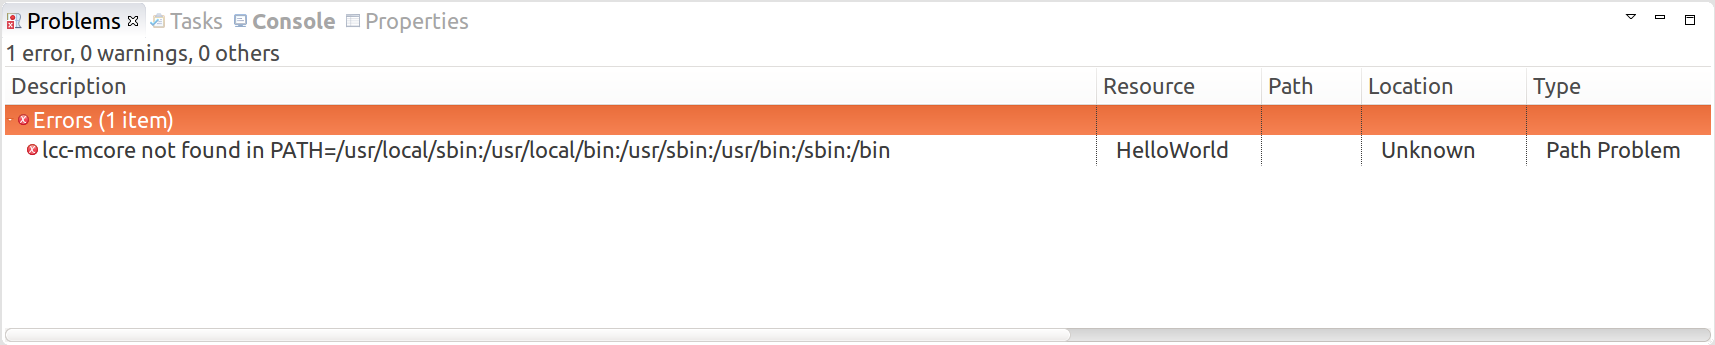
\includegraphics[scale=0.25]{compiler/patherror.png}
		\caption{Die Eclipse Problems View zeigt, dass das Program lcc-mcore nicht gefunden wurde im Pfad.}
		\captionsetup{margin=0cm,font={footnotesize}}
		\label{fig:patherror}
\end{figure}

In der Installationsanleitung im Anhang befinden sich alle Schritte, welche notwendig sind um die Entwicklungsumgebung zu installieren.

